% !TeX program = xelatex
\documentclass[UTF8,12pt,a4paper]{ctexart}

% ---------- 常用宏包 ----------
\usepackage[a4paper,margin=2.5cm]{geometry}
\usepackage{amsmath,amssymb,amsthm,mathtools,bm}
\usepackage{enumitem}
\usepackage{fancyhdr}
\usepackage{lastpage}
\usepackage{xcolor}
\usepackage{hyperref}
\usepackage{tikz}

% ---------- 请修改这里 ----------
\newcommand{\coursename}{工程硕士数学}
\newcommand{\homeworknumber}{HW2}
\newcommand{\studentname}{陈天乐}
\newcommand{\studentid}{[student ID removed]}
\newcommand{\classinfo}{深微硕6班}
\newcommand{\submissiondate}{\today}

% ---------- 页面设置 ----------
\setlength{\parindent}{2em}
\setlength{\parskip}{0.35em}
\linespread{1.25}

\pagestyle{fancy}
\fancyhf{}
\lhead{\coursename}
\chead{\homeworknumber}
\rhead{\studentname}
\cfoot{第 \thepage\ 页，共 \pageref{LastPage} 页}
\renewcommand{\headrulewidth}{0.4pt}

\hypersetup{
  colorlinks=true,
  linkcolor=blue,
  urlcolor=blue,
  pdftitle={\coursename—\homeworknumber},
  pdfauthor={\studentname}
}

% ---------- 题目与解答环境 ----------
\newcounter{problem}
\newenvironment{problem}[1][]
  {\refstepcounter{problem}\par\medskip
   \noindent\textbf{\large 题目 \theproblem\if\relax\detokenize{#1}\relax\else\quad #1\fi}
   \par\smallskip\noindent}
  {\par\medskip}

\newenvironment{solution}
  {\noindent\textbf{解：}\quad}
  {\hfill$\square$\par\medskip}

\newenvironment{proofcn}
  {\noindent\textbf{证明：}\quad}
  {\hfill$\blacksquare$\par\medskip}

% 常用命令
\newcommand{\R}{\mathbb{R}}
\newcommand{\norm}[1]{\left\lVert #1\right\rVert}
\newcommand{\abs}[1]{\left\lvert #1\right\rvert}
\DeclareMathOperator{\rank}{rank}
\DeclareMathOperator{\diag}{diag}

\begin{document}

% ---------- 标题 ----------
\begin{center}
  {\LARGE\bfseries \coursename}\par
  \vspace{0.4em}
  {\Large \homeworknumber}\par
  \vspace{1em}
  \begin{tabular}{rl@{\qquad}rl}
    姓名：& \studentname & 学号：& \studentid \\
    班级：& \classinfo   & 日期：& \submissiondate
  \end{tabular}
\end{center}

\vspace{0.5em}
\hrule
\vspace{1em}

% ---------- 正文示例 ----------
\begin{problem}[]
设 $A\in\mathbb{R}^{n\times n}$，设 $A$ 对称正定，记
\[
\|x\|_A = (Ax,x)^{\frac12},\quad \forall x\in\mathbb{R}^n,
\]
试证 $\|x\|_A$ 为 $\mathbb{R}^n$ 上的一种范数。(提示:可以从向量范数定义证明,也可利用 $A$ 对称正定,一定存在 $B\in\mathbb{R}^{n\times n}$,使 $A=BB^T$.)\end{problem}

\begin{proofcn}

对于$ \forall x\in \mathbb{R}^n $，
\[
\|x\|_A=(Ax,x)^{\frac12}\ge0
\]

并且
\[
\|x\|_A=0\Rightarrow x^TAx=0\xRightarrow{\text{A对称正定}} x=0
\]

对于$ \forall \alpha\in \mathbb{R} $，
\[
\|\alpha x\|_A=(A\alpha x,\alpha x)^{\frac12} =|\alpha| (Ax,x)^{\frac12} = |\alpha|\|x\|_A
\]

对于$ \forall x,y\in \mathbb{R}^n $，
\[
\|x+y\|_A ^2= (x^T+y^T)A(x+y) = (x^TAx+y^TAy)+(x^TAy+y^TAx)
\]

\[
\because x^TAy=y^TAx\Rightarrow \|x+y\|_A ^2=\|x\|_A^2+\|y\|_A^2+2x^TAy
\]

\[
\because \mbox{A对称正定}\Rightarrow \mbox{一定存在 $B\in\mathbb{R}^{n\times n}$,使 $A=BB^T$}
\]

\[
\therefore |x^TAy|=|(B^Tx)^T(B^Ty)|\le \|B^Tx\|_2\|B^Ty\|_2 = \|x\|_A\|y\|_A
\]

\[
\therefore \|x+y\|_A ^2\le \|x\|_A^2+\|y\|_A^2+2\|x\|_A\|y\|_A=(\|x\|_A+\|y\|_A)^2
\]

\[
\therefore \|x+y\|_A \le \|x\|_A+\|y\|_A
\]

综上，$\|x\|_A$满足正定性、齐次性和三角不等式，故$\|\cdot\|_A$是$\mathbb{R}^n$上的一种向量范数.

\end{proofcn}

\begin{problem}
设 $A=[a_{ij}]\in\mathbb{R}^{5\times5}$, $l_2=(0,0,2,-1,4)^T$,求 $L(-l_2)=I-l_2e_2^T$ 和 $L(-l_2)A$.
\end{problem}

\begin{solution}

\[
L(-l_2)=I-l_2e_2^T=
\begin{bmatrix}
1 & 0 & 0 & 0 & 0\\
0 & 1 & 0 & 0 & 0\\
0 & 0 & 1 & 0 & 0\\
0 & 0 & 0 & 1 & 0\\
0 & 0 & 0 & 0 & 1
\end{bmatrix}
-
\begin{bmatrix}
0\\
0\\
2\\
-1\\
4
\end{bmatrix}
\begin{bmatrix}
0&1&0&0&0
\end{bmatrix}
=
\begin{bmatrix}
1 & 0 & 0 & 0 & 0\\
0 & 1 & 0 & 0 & 0\\
0 & -2 & 1 & 0 & 0\\
0 & 1 & 0 & 1 & 0\\
0 & -4 & 0 & 0 & 1
\end{bmatrix}
\]
\[
L(-l_2)A
=
\begin{bmatrix}
a_{11} & a_{12} & a_{13} & a_{14} & a_{15}\\
a_{21} & a_{22} & a_{23} & a_{24} & a_{25}\\
a_{31}-2a_{21} & a_{32}-2a_{22} & a_{33}-2a_{23} & a_{34}-2a_{24} & a_{35}-2a_{25}\\
a_{41}+a_{21} & a_{42}+a_{22} & a_{43}+a_{23}& a_{44}+a_{24} & a_{45}+a_{25}\\
a_{51}-4a_{21} & a_{52}-4a_{22} & a_{53}-4a_{23} & a_{54}-4a_{24} & a_{55}-4a_{25}
\end{bmatrix}
\]

\end{solution}

\begin{problem}[]
对称正定矩阵 $A=[a_{ij}]\in\mathbb{R}^{n\times n}$,试证:
\begin{enumerate}
    \item $a_{ii}>0,\ i=1,2,\dots,n$;
    \item 若 $i\ne j,\alpha\in\mathbb{R}$,则 $a_{ii}+2\alpha a_{ij}+\alpha^2a_{jj}>0$;
    \item 若 $i\ne j$,则 $a_{ij}^2<a_{ii}a_{jj}$;
    \item $A$ 的绝对值最大元素在对角线上.
\end{enumerate}
\end{problem}

\begin{proofcn}
\begin{enumerate}
\item[1.]
\[
A\mbox{对称正定}\Rightarrow e_i^TAe_i=a_{ii}>0,\forall i=1,2,...,n
\]

\item[2.]
取$x=e_i+\alpha e_j$,
\[
A\mbox{对称正定}\Rightarrow x^TAx=a_{ii}+2\alpha a_{ij}+\alpha^2 a_{jj}>0
\]

\item[3.]
由2.得：
\[
\forall \alpha \in \mathbb{R}\mbox{且}i\neq j, a_{jj}\alpha^2+2a_{ij}\alpha +a_{ii}>0\mbox{恒成立}
\]
\[
\because a_{jj}>0\Rightarrow \Delta=4a_{ij}^2-4a_{ii}a_{jj}<0\Rightarrow a_{ij}^2<a_{ii}a_{jj} 
\]

\item[4.]
设$\max(a_{ii})=a_{kk}$，由3.得：
\[
a_{ij}^2<a_{ii}a_{jj}<max(a_{ii})^2=a_{kk}^2\Rightarrow |a_{ij}|<a_{kk}
\]

故A的绝对值最大元素在对角线上

\end{enumerate}

\end{proofcn}

\begin{problem}[]
确定 $a$ 的取值范围,使
\[
A=
\begin{bmatrix}
2 & a & -1\\
a & 2 & 1\\
-1 & 1 & 4
\end{bmatrix}
\]
是对称正定矩阵.
\end{problem}

\begin{solution}

若A是对称正定矩阵，那么它所有的顺序主子式都应大于0：
\[
\Delta_1 = 2 >0
\]

\[
\Delta_2=
\begin{vmatrix}
2&a\\
a&2
\end{vmatrix}
=4-a^2 >0\Rightarrow a \in (-2,2)
\]

\[
\Delta_3 = \det(A)=2\cdot 7 - a(4a+1)-(a+2)=-4a^2-2a+12=-2(2a-3)(a+2)>0\Rightarrow a\in(-2,\frac32)
\]

综上，$a\in (-2,\frac32)$
\end{solution}




\begin{problem}
设 $x>0,y>0$.确定 $(x,y)$ 所在区域,使
\[
A=
\begin{bmatrix}
3 & 2 & y\\
x & 5 & y\\
2 & 1 & x
\end{bmatrix}
\]
是严格对角占优矩阵,在 $xOy$ 坐标平面上画出此区域.
\end{problem}

\begin{solution}

\[
\begin{cases}
|y|+2<3\\
|x|+|y|<5\\
|x|>3 \\
x>0\\
y>0
\end{cases}
\Rightarrow
\begin{cases}
0<y<1\\
3<x<5-y
\end{cases}
\]
在$xOy$坐标平面的区域$\Omega$为：
\begin{center}
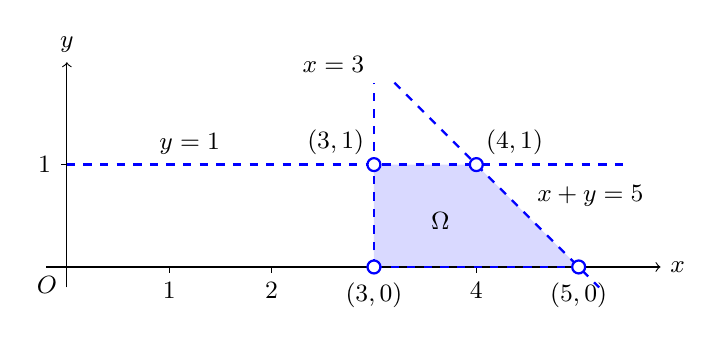
\begin{tikzpicture}[scale=1.3, font=\small]

  % 所求区域：0<y<1，3<x<5-y
  \fill[blue!15]
    (3,0) -- (5,0) -- (4,1) -- (3,1) -- cycle;

  % 坐标轴
  \draw[->] (-0.2,0) -- (5.8,0) node[right] {$x$};
  \draw[->] (0,-0.2) -- (0,2) node[above] {$y$};
  \node[below left] at (0,0) {$O$};

  % 坐标刻度
  \foreach \t in {1,2,4}{
    \draw (\t,0) -- (\t,-0.06);
    \node[below] at (\t,-0.06) {$\t$};
  }
  \draw (0,1) -- (-0.06,1);
  \node[left] at (-0.06,1) {$1$};

  % 边界均不包含，因此使用虚线
  \draw[blue, dashed, thick]
    (3,0) -- (3,1.8);
  \node[above left] at (3,1.8) {$x=3$};

  \draw[blue, dashed, thick]
    (0,1) -- (5.5,1);
  \node[above] at (1.2,1) {$y=1$};

  \draw[blue, dashed, thick]
    (3.2,1.8) -- (5.2,-0.2);
  \node[above right] at (4.5,0.5) {$x+y=5$};

  \draw[blue, dashed, thick]
    (3,0) -- (5,0);

  % 空心顶点：表示顶点不包含
  \foreach \p in {(3,0),(5,0),(4,1),(3,1)}{
    \draw[blue, thick, fill=white]
      \p circle[radius=1.8pt];
  }

  % 顶点标注
  \node[below]       at (3,-0.06) {$(3,0)$};
  \node[below]       at (5,-0.06) {$(5,0)$};
  \node[above right] at (4,1)     {$(4,1)$};
  \node[above left]  at (3,1)     {$(3,1)$};

  % 区域标记
  \node at (3.65,0.45) {$\Omega$};

\end{tikzpicture}
\end{center}

\end{solution}

\begin{problem}[]
设
\[
A=
\begin{bmatrix}
a & 1 & 0\\
b & 2 & 1\\
0 & 1 & 2
\end{bmatrix},
\]
分别求出所有 $a,b$ 的值,使得:
\begin{enumerate}
    \item $A$ 奇异;
    \item $A$ 严格对角占优;
    \item $A$ 对称正定.
\end{enumerate}
\end{problem}

\begin{solution}
\begin{enumerate}
  \item [1.]
  若A奇异，则：
  \[
  \det(A)=3a-2b=0\Rightarrow a=\frac{2b}{3}, b\in\mathbb{R}
  \]
  \item [2.]
    若A严格对角占优，则：

  \[
  \begin{cases}
   |a|>1\\
   |b|+1<2
  \end{cases}
  \Rightarrow 
  \begin{cases}
    a>1\mbox{或}a<-1\\
    -1<b<1
  \end{cases}
  \]
  \item [3.]
  若A对称正定，那么A的所有顺序主子式均大于0：
  \[
  \begin{cases}
  \Delta_1 = a >0\\
  \Delta_2 = 
  \begin{vmatrix}
a&1\\
b&2
\end{vmatrix}
  =2a-b>0\\
  \Delta_3 = \det(A)=3a-2b>0\\
  b=1
\end{cases}
\Rightarrow
\begin{cases}
  b=1\\
  a>\frac23
\end{cases}
\]
  
\end{enumerate}

\end{solution}


\end{document}
